\begin{frame}
    \frametitle{Downblending HEU is a potential source of HALEU}
    To meet the fourth objective, I modeled the neutronics of 
    different HALEU compositions in the Xe-100 and MMR.
    \begin{itemize}
        \item Consider pure HALEU ($^{235}$U and $^{238}$U only)
              and HALEU from downblended \gls{EBR} 
              \cite{vaden_isotopic_2018} and Y-12 
              \cite{nelson_foreign_2010} stockpiles
        \item Create Serpent \cite{leppanen_serpent_2013} models 
              for these two reactors
        \item Compare the performance of the fuels with respect to:
        \begin{itemize}
            \item \keff
            \item \betaEff
            \item Energy- and spatially dependent flux
            \item Fuel, coolant, moderator, and total reactivity
                  temperature feedback coefficients
        \end{itemize}
    \end{itemize}

\end{frame}

\begin{frame}
    \frametitle{Energy dependent neutron flux in Xe-100}
    \begin{figure}
        \centering 
        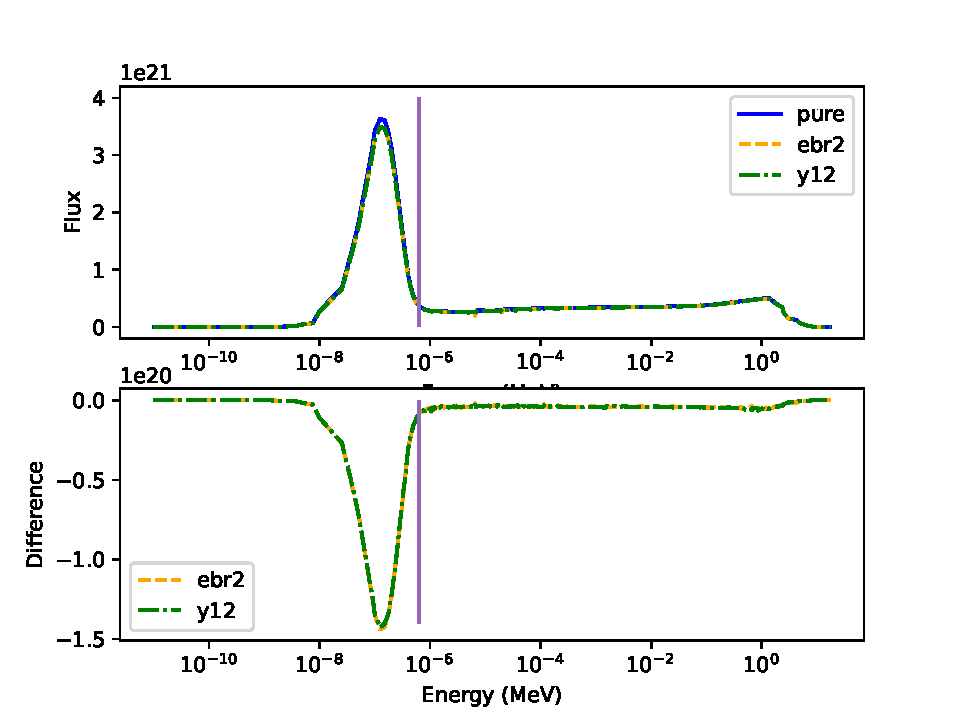
\includegraphics[scale=0.5]{xe100_mg_flux.pdf}
        \caption{Energy-dependent flux through the active region 
        of the Xe-100 core. The purple line is the delineation 
        between fast and thermal neutrons for this work.}
    \end{figure}
\end{frame}

\begin{frame}
    \frametitle{Spatitally-dependent netron flux in Xe-100}
    \begin{figure}
        \centering 
        \begin{subfigure}{0.49\textwidth}
            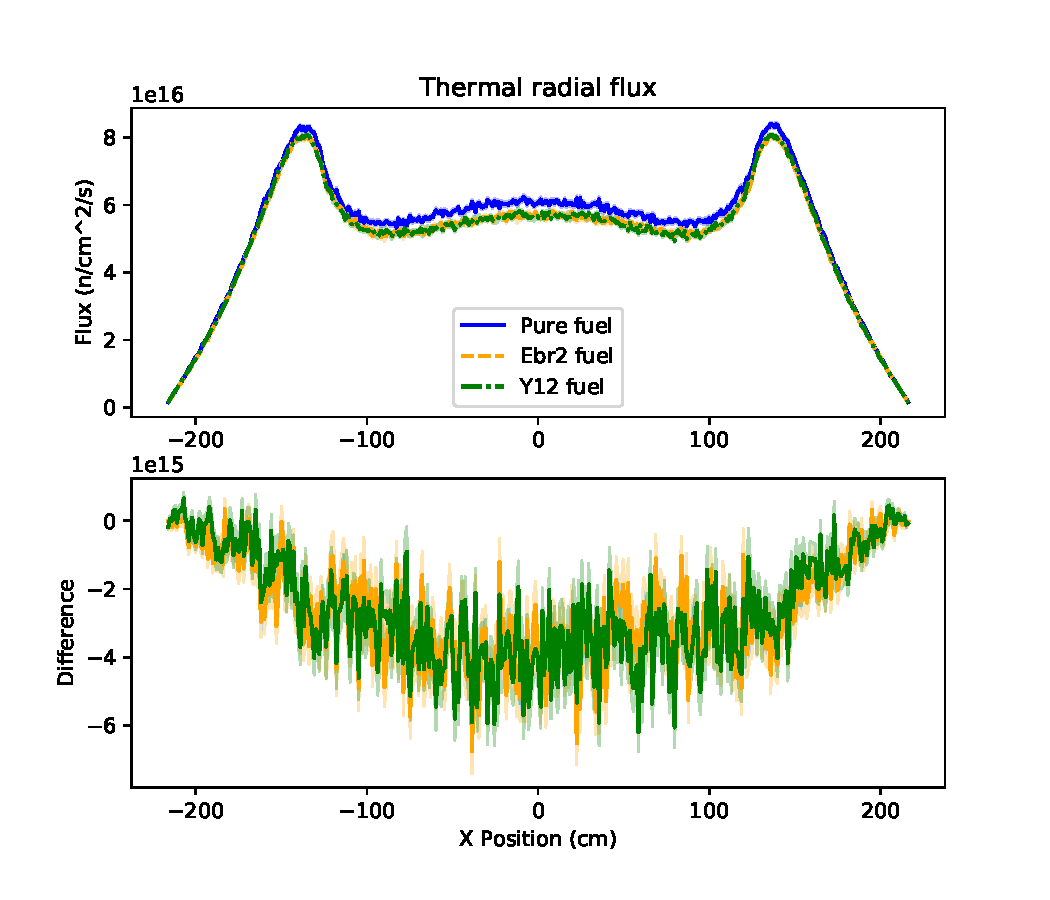
\includegraphics[width=\linewidth]{xe100_thermal_radial.pdf}
        \end{subfigure}
        \begin{subfigure}{0.49\textwidth}
            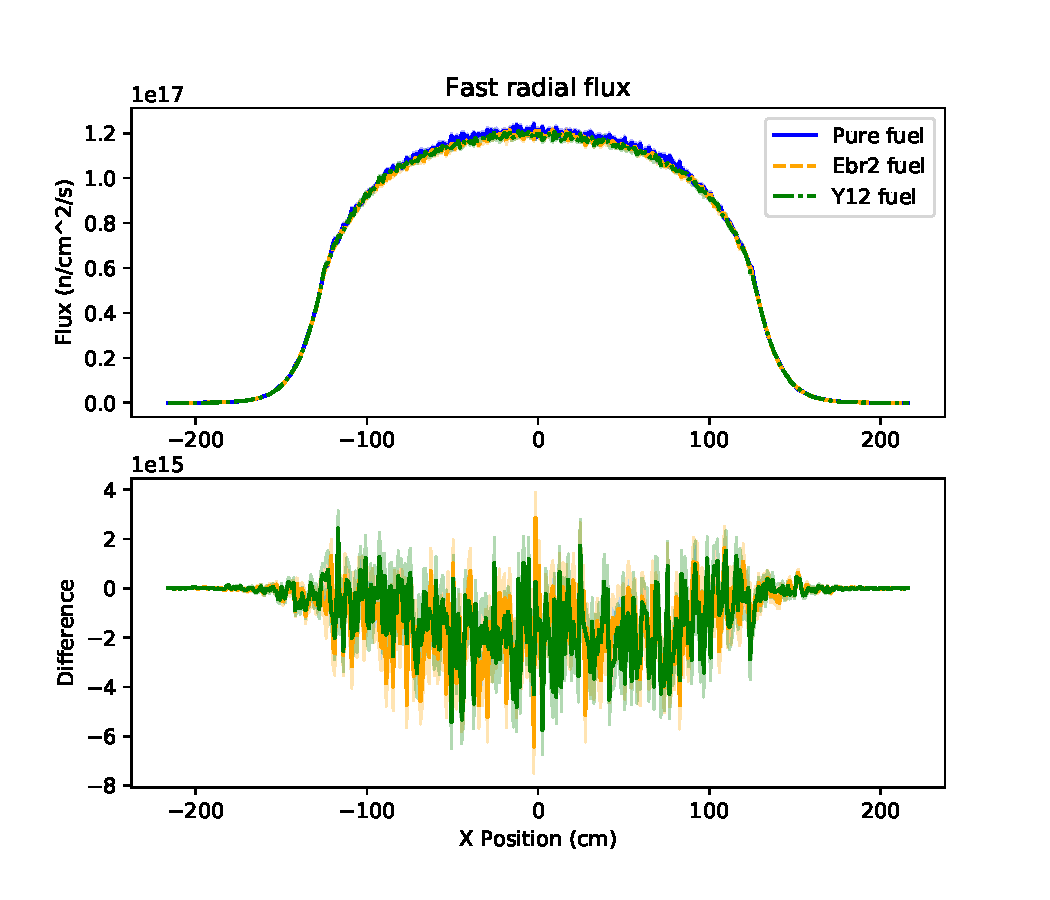
\includegraphics[width=\linewidth]{xe100_fast_radial.pdf}
        \end{subfigure}
        \caption{Radial fluxes through Xe-100.}
        \label{fig:xe100-flux}
    \end{figure}
\end{frame}